\documentclass[%
  chapterprefix=false,%
  open=right,%
  twoside=true,%
  paper=a4,%
  logofile={Figures/logo.png},%
  thesistype=master,%
  UKenglish,%
]{se2thesis}
\listfiles
\usepackage[ngerman,main=UKenglish]{babel}
\usepackage{blindtext}
\usepackage[%
  csquotes=true,%
  booktabs=true,%
  siunitx=true,%
  minted=true,%
  selnolig=true,%
  widowcontrol=false,%
  microtype=true,%
  biblatex=true,%
  cleveref=true,%
]{se2packages}

\addbibresource{ref.bib}

\usepackage{hyperref}
\usepackage[caption=false]{subfig}

\author{Gonzalo A. Oberreuter Álvarez}
\title{Master Thesis Proposal}
\degreeprogramme{Computer Science}
\matrnumber{0815}
\supervisor{Prof.\,Dr.~Gordon Fraser}
\external{}
\advisor{}
\department{Faculty of Mathematics and Informatics}
\institute{Chair of Software Engineering}
\location{Passau}

\begin{document}

\frontmatter

\maketitle

\iffalse{}

\authorshipDeclaration{}

\begin{abstract}
  An English abstract to the thesis. 
  TBD.\@
\end{abstract}

\begin{abstract}[german]
  Eine deutschsprachige Zusammenfassung der Arbeit.
  TBD.\@
\end{abstract}

\begin{acknowledgements}
  Some acknowledgements. 
  TBD.\@
\end{acknowledgements}

\tableofcontents

\fi

\mainmatter{}

\chapter{Introduction}

Software Testing is one of the key aspects of Software Developing while trying to ensure quality over a final product, regardless of the context in which the developing process is made.
This quality can be achieved by the insight provided by the result of the tests, and even because of the defects that can be encountered during the testing phase.
Nonetheless, even though coding different kinds of tests is a good practice, this is often ignored by new or inexpert developers, who also make this mistake half way by not getting a complete introspection   of their own code or, in other words, not getting a complete kind of test coverage.
As of 2017, a study by Trauch and Grabowski~\cite{DBLP:conf/icst/TrautschG17} presented that, over more than 4 million tests, most of them weren't correctly categorized (as unit test or not) and approximately half of them use mocking as a testing technique, which tells some aspects about the developing community of the projects in review. 
With this general idea into mind, is that researchers in the last decade   have put effort into autonomous test generation, the concept that implies the usage of different methods or techniques in order to identify patterns and generate test sets with little to zero   external intervention.
In 2015, empirical proof was found who showed the following statements about the usage of automated Java unit test generation:
\begin{itemize}
  \item It increases the general structural coverage.
  \item It does not lead to the detection of more faults.
  \item It affects negatively the ability to capture intended class behaviour.
\end{itemize}
according to Fraser et al~\cite{DBLP:journals/tosem/FraserSMAP15}.
The results of this study state fundamentaly that this behaviour  comes from the early stages of the tool in question, and proposes to put more work into the readability of generated tests and  the process of test making itself.

Although automatic test generation is achievable with no major problem for statically typed languages like Java~\cite{DBLP:journals/tse/FraserA13} or C, dynamically typed languages such as Python, Javascript or Lua enforce problems at the time of generating correct parameters for the execution of methods or function under test.
%Explain what a dynamically typed language is?
The major concern about the parameter generation, is that the lack of type information produces ambiguity for the heuristics of the tool at hand at the moment of synthesizing non-primitive types.
Also, the complexity of this object or callable types might produce runtime errors, which imply a local optima in the search landscape of the test representation~\cite{DBLP:conf/sigsoft/0001O00D21} and therefore an upper bound for coverage.

Within the scope of Python testing, Pynguin~\cite{DBLP:conf/icse/LukasczykF22} is a test generation framework that applies various algorithms for input generation, such as DynaMOSA~\cite{DBLP:journals/tse/PanichellaKT18}, MIO~\cite{DBLP:conf/ssbse/Arcuri17}, MOSA~\cite{DBLP:conf/icst/PanichellaKT15}, random~\cite{DBLP:conf/icse/PachecoLEB07}, Whole Suite~\cite{DBLP:journals/tse/FraserA13}, and Whole Suite with archive~\cite{DBLP:journals/ese/RojasVAF17}.

\begin{figure}[tb]
  \centering
  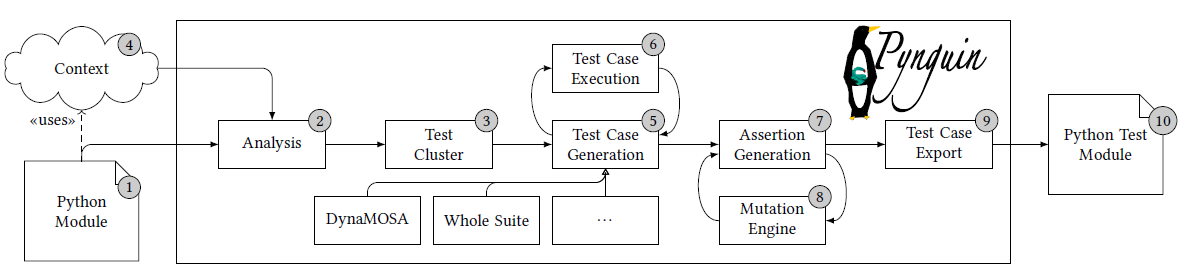
\includegraphics[width=.99\textwidth]{Figures/pynguin.png}
  \caption{Pynguin Structure}\label{fig:pyn}
\end{figure}

Its structure is presented in Figure~\ref{fig:pyn} and consists of 10 autonomous steps that work in the following manner
\begin{enumerate}
  \item The unit test generation process starts with the input of a user defined python module, or directory cont
\end{enumerate}
%Is this plagio?
At the time of its original release (25th of July 2020), Pynguin was a state of the art open source tool that has made the first step of a sequence of subsecuent researches about how to improve the performance and functionalities of Pynguin itself, including CodaMOSA~\cite{DBLP:conf/icse/LemieuxILS23} or PyLC~\cite{DBLP:conf/sac/SalariEAS23}

This recent new extensions of Pynguin and the aforementioned problem at the time of generating complex object inputs are the principal motivations of this thesis and the related and future work to it.

\iffalse{}
\begin{summary}{Structure}
\begin{itemize}
  \item test generation CHECK
  \item test generation in dynamic languages and it's difficulties CHECK
  \item pynguin and its accomplishments
\end{itemize}
\end{summary}

\fi


\chapter{Proposal}

The original Pynguin research paper~\cite{DBLP:conf/icse/LukasczykF22} stated that after the test generation of 118 Python modules, the average branch coverage over all algorithms was $66.8\%$, which leads to think that improvement is possible.
%talk about how coverage isn't everything?
The current Master's thesis proposes an addition to the original structure of Pynguin~(see~Figure~\ref{fig:pyn}), specifically to sections (5) and (2) by developing
a Graph-Based Object Synthesis approach~\cite{DBLP:conf/sigsoft/0001O00D21} and optionaly the usage of an external type inference module respectively, in order to diminish the branch coverage gap and try to generate more complex test suites.

What the Graph-Based heuristic proposed by Lin et al.~\cite{DBLP:conf/sigsoft/0001O00D21} does, is generate a object construction graph (OCG) from a previous code slicing, performed from the program dependency graph and a specific target branch as criteria.
This branch must be selected from those who have not reached their full coverage, or are ``non-trivial'', and the depth of the intraprocedural dependency should be set as a arbitrary level $t_{\text{dep}}$.
\textbf{Some explanation of the representation of code by Pynguin and its relevance to the algorithm should be explained.}
Then, this OCG is used to generate a code template that should be either translated directly into the test code representation of Pynguin or an intermediate form.
This previous idea was completely implemented in and for Java, which means that part of the work to be done is to ideate a new Python representations of the OCG.\@
The usage of a external type inference library is mentiones as optional in the hypotethical case of the branch coverage improvement not being as substantial in Pynguin as the one obtained while experimenting over EvoObj, the new instance of EvoSuit.
After all the coding is done, a study of the extension will be made through the selection of arbiotrary set of Python module, being these either the original research paper's or a new set that ensures the explicit type of object inputs and a ratio of this kind of inputs of more than $50\%$.
The final purpose of the thesis is to obtain an effect size over the coverage results between Pynguin and the proposed extension either equal or bigger to the ones obtained between EvoSuit and EvoObj, being this greater than an average of $0.30$ over ¿all? possible algorithms in the different time budgets.



\begin{summary}{Objectives}
\centering\textbf{General Objective}
\begin{itemize}
\item  Develop a Pynguin extension that generates graph-based complex object inputs and increases the effect size of the branch coverage results by a factor of $0.30$
\end{itemize}
\centering\textbf{Secondary Objectives}
\begin{itemize}
\item  Pick a set of adecuate Python modules to prove the effectiveness of the Pynguin extension
\item (Optional) Integrate Pynguin with an external type inference library
\end{itemize}
\end{summary}

\chapter{State of the Art}

\begin{itemize}
  \item state of the unit test generation
  \begin{itemize}
    \item EvoSuite~\cite{DBLP:conf/sigsoft/FraserA11}
  \end{itemize}
  \item state of the unit test generation in dynamic languages
  \begin{itemize}
    \item JSEFT(JS)~\cite{DBLP:conf/icst/Mirshokraie0P15}
    \item NxtUnit(GO)~\cite{DBLP:conf/ease/WangMCGSP23}
  \end{itemize}
  \item state of the unit test generation in python
  \begin{itemize}
    \item CodaMOSA~\cite{DBLP:conf/icse/LemieuxILS23}
    \item PBT-GPT~\cite{DBLP:journals/corr/abs-2307-04346}
    \item CodeT~\cite{DBLP:journals/corr/abs-2207-10397}
    \item MutAP~\cite{DBLP:journals/corr/abs-2308-16557}
    \item LExecutor~\cite{DBLP:journals/corr/abs-2302-02343}
    \item Mutester~\cite{DBLP:journals/corr/abs-2307-00404}
    \item ChatGPT~\cite{li2023nuances}
    \item PyLC~\cite{DBLP:conf/sac/SalariEAS23}
  \end{itemize}
\end{itemize}

Comments on the state of the art

\backmatter{}

\printbibliography{}

\end{document}
